\documentclass{amia}
\usepackage{graphicx}
\usepackage[labelfont=bf]{caption}
\usepackage[superscript,nomove]{cite}
\usepackage{color}
\usepackage{wrapfig}
\usepackage{hyperref}
\usepackage[normalem]{ulem}

\setlength{\voffset}{-.5in}

\begin{document}

\title{Creating RDF Data on Trauma Care Organizations from Questionnaires}

\author{Joseph R. Utecht, BA$^{1}$, Mathias Brochhausen, PhD$^{1}$}

\institutes{
    $^1$University of Arkansas for Medical Science, Little Rock, AR, USA\\
}

\maketitle

\section*{Background}

Assessment of trauma systems and trauma centers positively affects patient outcomes \cite{ref1, ref2}.
However, assessment of these organizations often falls short because of a lack of comparability regarding components and their implementation.
The CAFE project(\href{https://cafe-trauma.com}{https://cafe-trauma.com}) aims to provide a web-based self-assessment environment for this domain. 
To this end we develop a user-friendly questionnaire allowing users to enter data and compare organizational components in real time .
This poster describes our methodology to create semantically-rich data based on user-friendly, web-based questionnaires.
The main innovation is that, in addition to storing answers in a relational database, our survey system also generates RDF (\href{https://www.w3.org/RDF}{https://www.w3.org/RDF}) statements representing the portion of reality that the answer reports.

\section*{Methods}
To support our requirement of allowing user-friendly data entry we developed a tool to create traditional web questionnaires.
To prevent any interruption for the user while the server processes previous answers we chose to build the interface as a separate web application in Angular2 (\href{https://angular.io}{https://angular.io}).
To provide semantically-rich data the server-side component will not only record the answer in a relational database (RDB), but simultaneously create a pre-configured RDF representation of the answer in a triplestore.

\section*{Results}
\begin{wrapfigure}{r}{0.3\textwidth}
  \begin{center}
    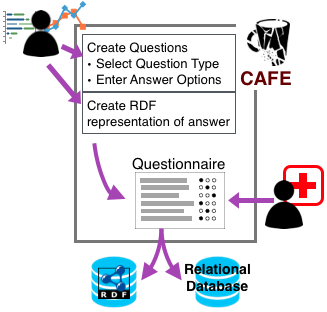
\includegraphics[width=0.28\textwidth]{pics/cafe_process6.png}
  \end{center}
  \caption{CAFE Process.}
  \label{cafe_process}
\end{wrapfigure}

The result of this work is available on Github (\href{https://github.com/cafe-trauma}{https://github.com/cafe-trauma}). Fig. 1 shows the steps of acquiring RDF data through a questionnaire built using our tool. 
The first step is the creation of the questions and the definition of the RDF representation for the answers.
The tool then builds a traditional web questionnaire.
As respondents answer questions their answers are recorded in a RDB and the RDF representation will be created in a triplestore.

For example, if the question ``Does your trauma center have a trauma registrar?" is answered affirmatively, RDF statements are created to represent the individual trauma registrar and the individual trauma center in question, and the fact that the trauma registrar is an organizational member of that trauma center.
At the same time it records the simple answer ``yes" in the RDB.

From the user's point of view the questionnaire does not differ in any way from a typical web questionnaire.
The benefit of this method is that the data about a respondent's organization is available in a format that allows integration with rich semantic resources. 
In the CAFE project we use the OWL ontology OOSTT \cite{ref3} to integrate knowledge about trauma systems and trauma centers. 

\section*{Acknowledgements}
The research presented in this paper is funded by the National Institute of General Medical Sciences of the National Institutes of Health under award number \textbf{1R01GM111324}.

\makeatletter
\renewcommand{\@biblabel}[1]{\hfill #1.}
\makeatother

\bibliographystyle{unsrt}
\begin{thebibliography}{1}
\setlength\itemsep{-0.1em}

\bibitem{ref1}
T.L.Sanddal,T.J.Esposito,J.R.Whitney,D.Hartford,P.P.Taillac, N. C. Mann NC, et al.. "Analysis of preventable trauma deaths and opportunities for trauma care improvement in Utah," J Trauma. 2011 Apr;70(4):970-7.

\bibitem{ref2}
T. J. Esposito, T. L. Sanddal, S. A. Reynolds, N. D. Sanddal, "Effect of a voluntary trauma system on preventable death and inappropriate care in a rural state," J Trauma, 2003, 54(4), 663-670.

\bibitem{ref3}
Utecht J, Judkins J, Colvin T Jr., et al. OOSTT: a Resource for Analyzing the Organizational Structures of Trauma Centers and Trauma Systems. CEUR Workshop Proc. 2016 Aug;1747. \href{http://ceur-ws.org/Vol-1747/IT504_ICBO2016.pdf}{http://ceur-ws.org/Vol-1747/IT504\_ICBO2016.pdf}


\end{thebibliography}

\end{document}
